\clearpage % Rozdziały zaczynamy od nowej strony.

\section{Architektura systemu}

W tym rozdziale zostanie przedstawiona szczegółowa architektura projektowanego systemu. Celem tego rozdziału jest dostarczenie kompleksowego przeglądu wszystkich kluczowych komponentów, ich wzajemnych zależności, a także sposobu ich integracji.

\subsection{Podział na mikroserwisy}

Część serwerowa systemu została podzielona na mikroserwisy zgodnie z wcześniej wydzielonymi Ograniczonymi Kontekstami. Dodatkowo poza serwisami związanych z Ograniczonymi Kontekstami, zostały wydzielone serwisy wspólne, które są wykorzystywane przez pozostałe elementy systemu. Są to:

\begin{itemize}

    \item \textbf{Dostawy} (ang. \textit{deliveries}) - implementacja kontekstu "Dostawa",
    \item \textbf{Zamówienia} (ang. \textit{orders}) - implementacja kontekstu "Zamówienie",
    \item \textbf{Płatności} (ang. \textit{payments}) - implementacja kontekstu "Płatność",
    \item \textbf{Restauracje} (ang. \textit{restaurants}) - implementacja kontekstu "Restauracja",
    \item \textbf{Zapytania} (ang. \textit{queries}) - serwis odpowiedzialny za budowanie bazodanowych projekcji danych oraz obsługę zapytań. Jest wykorzystywany przez wszystkie pozostałe serwisy oraz część kliencką systemu,
    \item \textbf{Sagi} (ang. \textit{sagas}) - serwis odpowiedzialny za obsługę/orkiestrację długo trwających procesów biznesowych. Implementuje wzorzec Saga. Jest wykorzystywany przez wszystkie pozostałe serwisy.

\end{itemize}

Wydzielono również moduł niebędący mikroserwisem, a jedynie biblioteką, która jest wykorzystywana przez wszystkie pozostałe serwisy. Jest to \textbf{Wspólny kod} (ang. \textit{shared}), który zawiera wspólne dla wszystkich serwisów klasy, interfejsy, konfiguracje itp.

\subsection{Model C4 systemu}

W celu przedstawienia architektury systemu w sposób zrozumiały i przejrzysty, został wykorzystany model C4.

Model C4 \cite{c4} (Context, Containers, Components, Code) to metoda wizualizacji architektury oprogramowania, zaprojektowana przez Simona Browna, która skupia się na dekompozycji systemu na różne poziomy abstrakcji. Model ten zaczyna od Kontekstu (poziom 1), pokazując zewnętrzne zależności systemu, przechodzi przez Kontenery (poziom 2), ukazujące główne części systemu (np. aplikacje webowe, bazy danych), aż do Komponentów (poziom 3), przedstawiających wewnętrzną budowę poszczególnych pojemników, kończąc na Kodzie (poziom 4), który pokazuje szczegóły implementacji. Model ten jest szeroko stosowany w projektowaniu i dokumentacji architektury oprogramowania, pozwalając na jasne i spójne przedstawienie skomplikowanych systemów.

Pierwszym poziomem modelu C4 jest \textbf{Kontekst} (ang. \textit{Context}), który przedstawia zewnętrzne zależności systemu. Został on przedstawiony na rysunku \ref{fig:c4context}.

\begin{figure}[!h]
    \centering 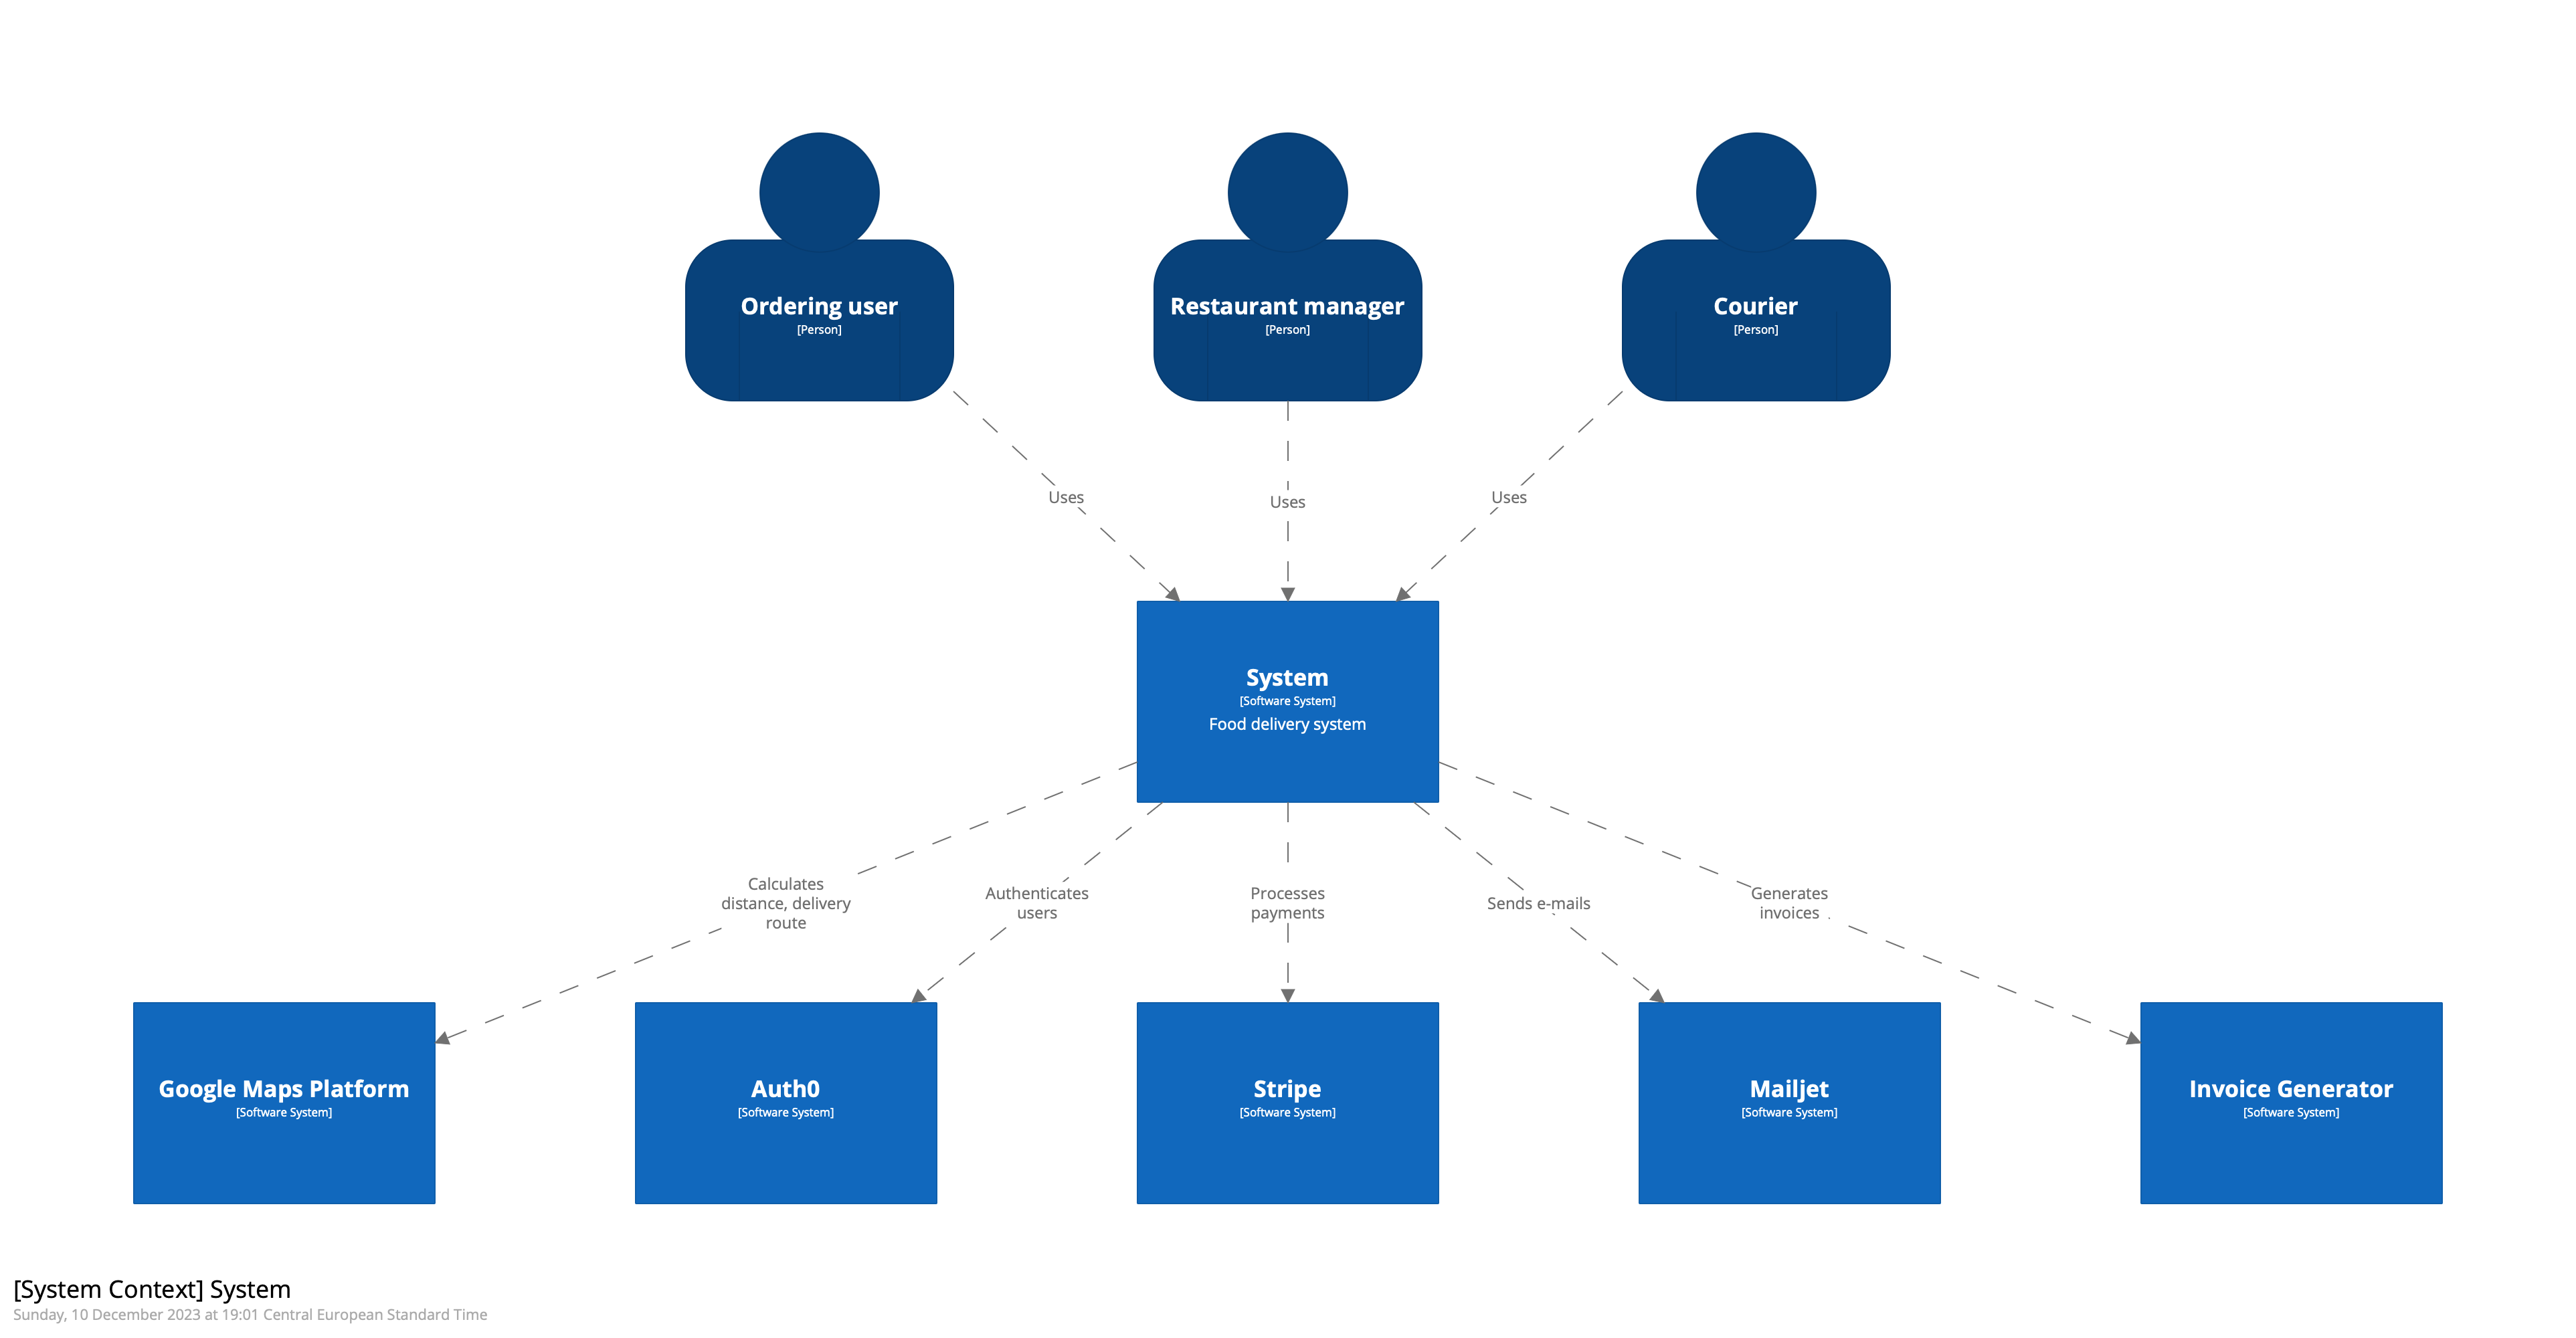
\includegraphics[width=1.0\linewidth]{c4context.png}
    \caption{Model C4 systemu - Kontekst}
    \label{fig:c4context}
\end{figure}

Na poziomie Kontekstu zostały przedstawione zewnętrzne systemy, z którymi system wchodzi w interakcję, a także użytkownicy systemu.

Drugim poziomem modelu C4 są \textbf{Kontenery} (ang. \textit{Containers}), które przedstawiają główne części systemu. Został on przedstawiony na rysunku \ref{fig:c4containers}.

\begin{figure}[!h]
    \centering 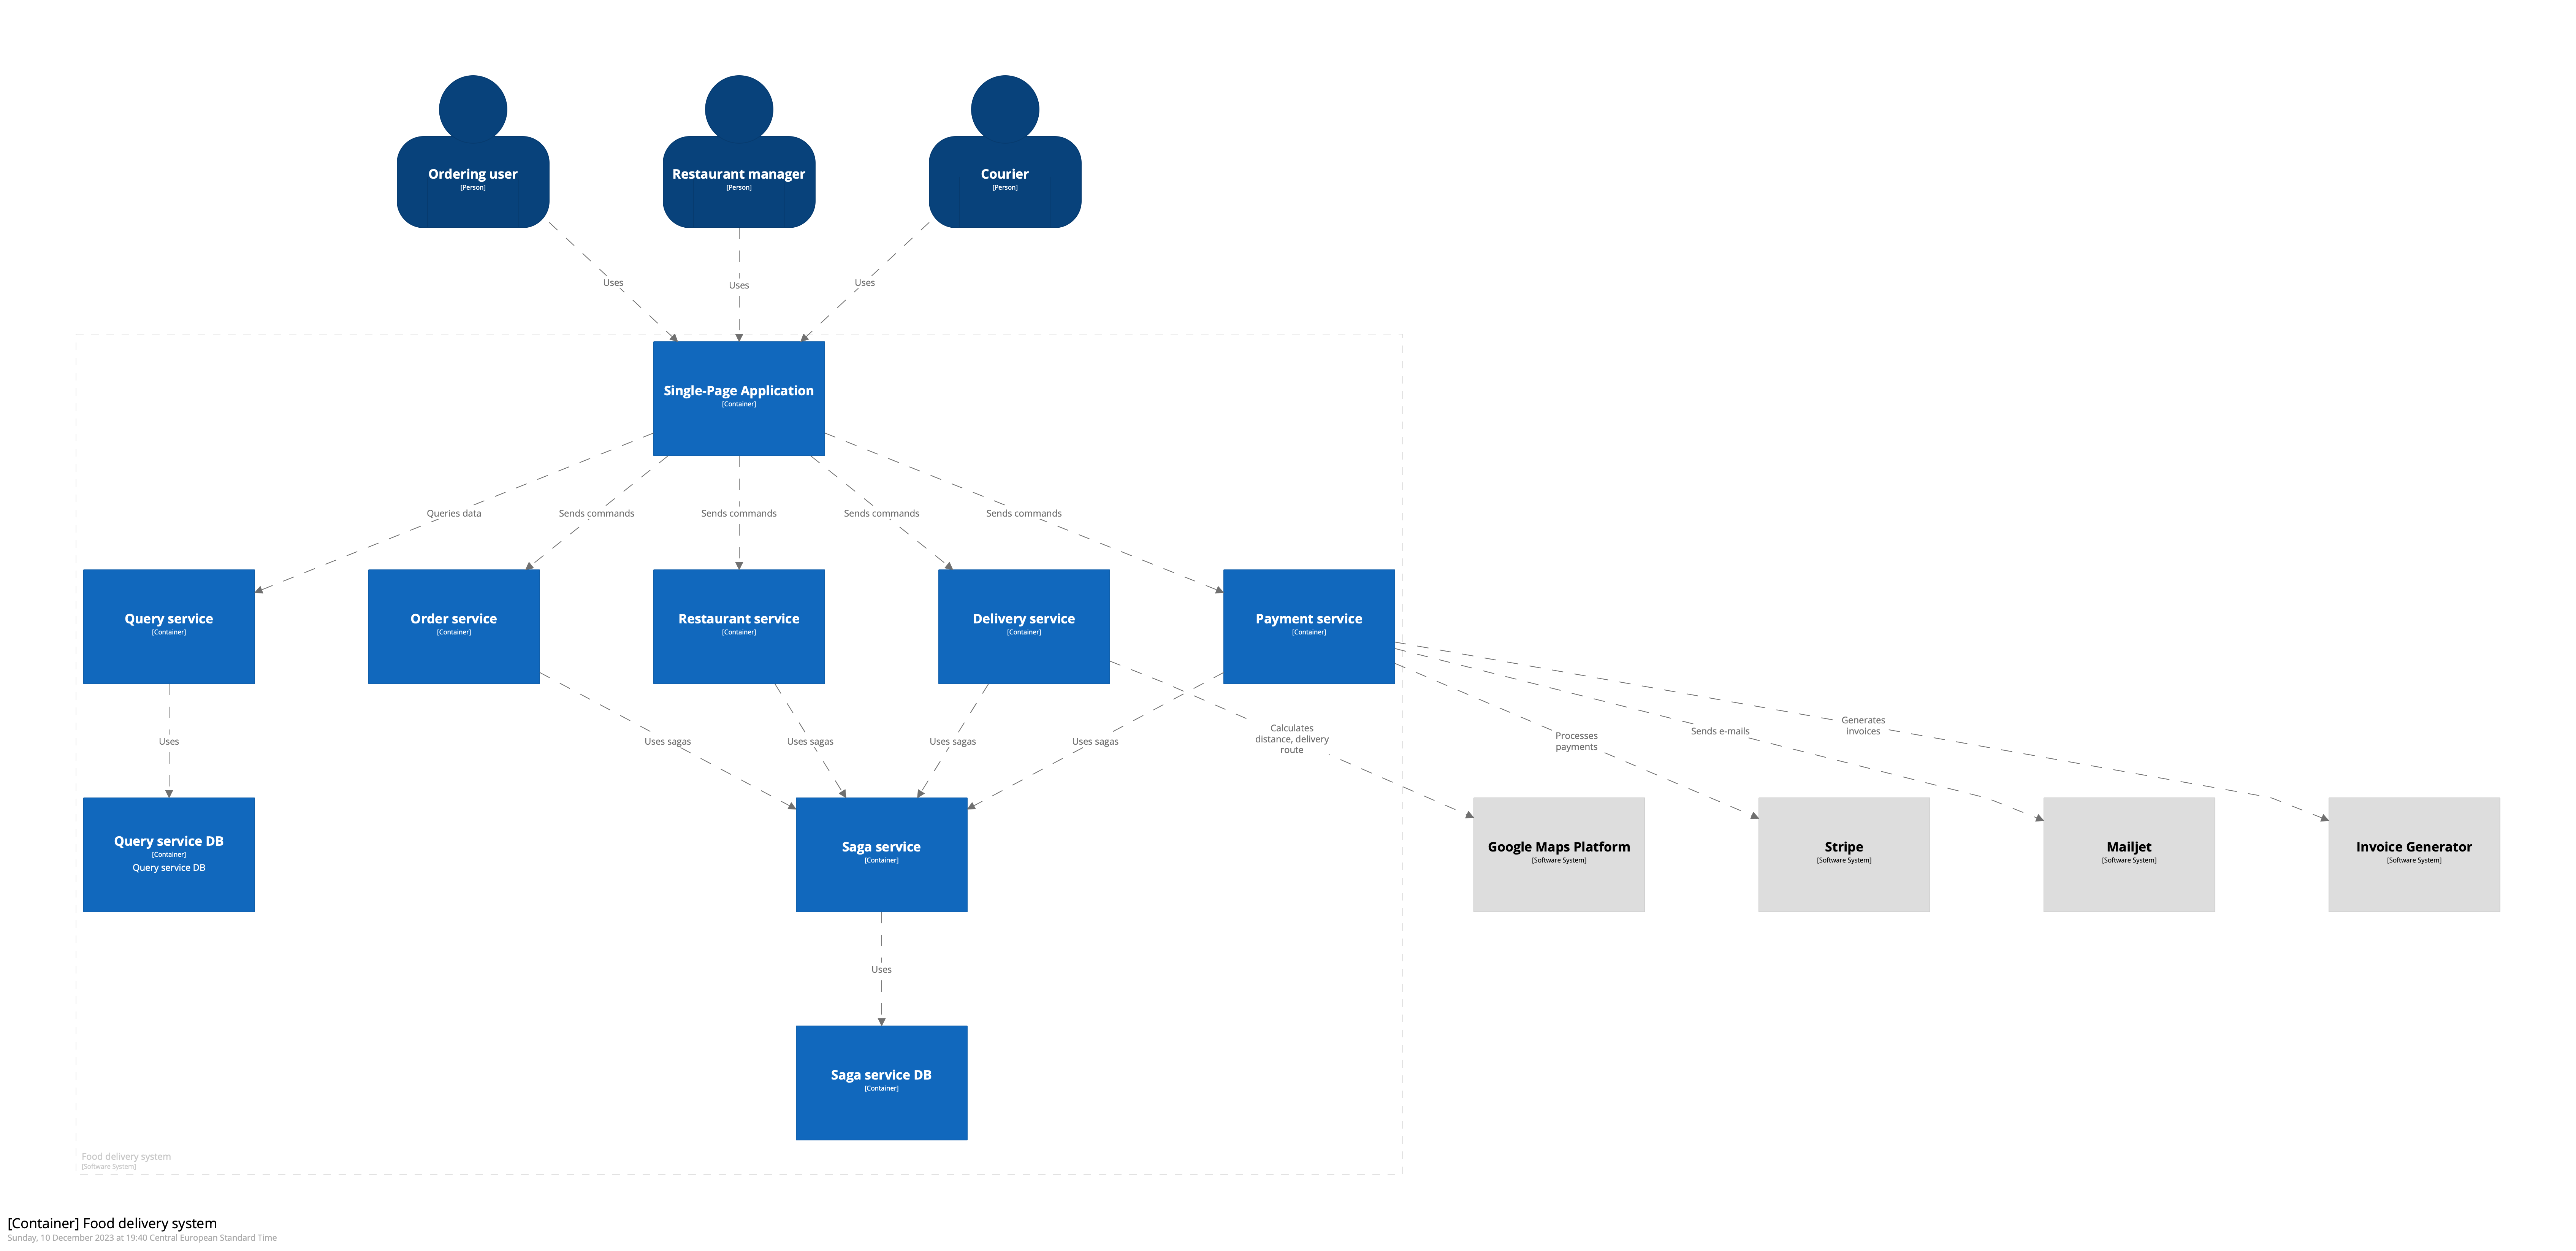
\includegraphics[width=1.0\linewidth]{c4containers.png}
    \caption{Model C4 systemu - Kontenery}
    \label{fig:c4containers}
\end{figure}

Na poziomie Kontenerów zostały przedstawione poszczególne serwisy, które zostały wydzielone w ramach części serwerowej systemu.

Trzecim poziomem modelu C4 są \textbf{Komponenty} (ang. \textit{Components}), które przedstawiają wewnętrzną budowę poszczególnych Kontenerów. Nie zostały one przedstawione w niniejszej pracy, ze względu na zbyt dużą szczegółowość. 

Czwarty poziom modelu C4 to \textbf{Kod} (ang. \textit{Code}), który przedstawia szczegóły implementacji poszczególnych Komponentów.

\subsection{Protokoły i formaty komunikacji}

W celu zapewnienia komunikacji pomiędzy poszczególnymi komponentami systemu zostały wykorzystane następujące protokoły i formaty komunikacji:

\begin{itemize}

    \item \textbf{Protokół HTTP} (ang. \textit{Hypertext Transfer Protocol}) - protokół komunikacyjny używany do przesyłania danych w Internecie, działający na zasadzie żądania i odpowiedzi między klientem a serwerem, charakteryzujący się bezstanowością i różnorodnymi metodami żądań, takimi jak GET czy POST. Bezpieczna wersja protokołu, HTTPS, dodatkowo zapewnia szyfrowanie danych, zwiększając prywatność i bezpieczeństwo transmisji. W projekcie został wykorzystany do komunikacji pomiędzy częścią kliencką systemu a serwisami serwerowymi.

    \item \textbf{Styl REST} (ang. \textit{Representational State Transfer}) - styl architektury oprogramowania używany do projektowania sieciowych systemów aplikacji, oparty na bezstanowych żądaniach i odpowiedziach, wykorzystujący standardowe metody HTTP i formaty wymiany danych, takie jak JSON czy XML, do tworzenia skalowalnych i elastycznych interfejsów API. REST akcentuje prostotę komunikacji sieciowej, umożliwiając łatwą integrację między różnymi systemami w Internecie.
    
    \item \textbf{Protokół gRPC} (ang. \textit{gRPC Remote Procedure Call}) - nowoczesny, otwartoźródłowy protokół zdalnego wywoływania procedur, opracowany przez Google, który umożliwia wydajną, szybką i bezpieczną komunikację między mikrousługami. Wykorzystuje format wymiany danych Protocol Buffers (Protobuf) \cite{protobuf} i jest oparty na modelu klient-serwer, wspierając funkcje takie jak dwustronna komunikacja strumieniowa, kontrola przepływu i uwierzytelnienie oparte na certyfikatach TLS. W projekcie został wykorzystany do komunikacji pomiędzy serwisami a kolejką komunikatów oraz magazynem zdarzeń.

    \item \textbf{Format JSON} \cite{json} (ang. \textit{JavaScript Object Notation}) - lekki format wymiany danych, łatwy do czytania i pisania dla ludzi oraz prosty do parsowania i generowania dla maszyn, wykorzystujący tekstowe struktury do reprezentowania obiektowych danych, zazwyczaj składających się z par klucz-wartość i uporządkowanych list. Jest powszechnie stosowany w komunikacji internetowej, w szczególności w interfejsach REST API i konfiguracjach. W projekcie został wykorzystany do przesyłania danych pomiędzy częścią kliencką systemu a serwisami.
    
    \item \textbf{Format XML} (ang. \textit{Extensible Markup Language}) - elastyczny i rozszerzalny format danych oparty na znacznikach, zaprojektowany do przechowywania i transportu danych w sposób zarówno czytelny dla maszyn, jak i ludzi, często używany w różnorodnych aplikacjach internetowych i konfiguracjach systemowych. Charakteryzuje się ścisłą strukturą, z hierarchicznie uporządkowanymi elementami i atrybutami, co sprawia, że jest idealny do reprezentowania złożonych struktur danych. W projekcie został wykorzystany do serializacji i deserializacji wiadomości: zdarzeń, komend i zapytań.

\end{itemize}

\subsection{Persystencja danych i magazyn zdarzeń}

Z powodu zastosowania wzorców CQRS i Event Sourcing w części serwerowej systemu odpowiadającej za obsługę komend nie ma konieczności stosowania standardowej bazy danych. Zamiast tego zastosowano specjalistyczne rozwiązanie, które umożliwia przechowywanie zdarzeń w postaci strumieni zdarzeń (ang. \textit{event streams}). Jest to \textbf{Magazyn zdarzeń} (ang. \textit{event store}), który jest wykorzystywany przez wszystkie serwisy.

Zastosowanym magazynem zdarzeń jest Axon Server \cite{axonserver} od firmy AxonIQ. Jest to otwartoźródłowy, wysokowydajny i niezawodny magazyn zdarzeń, zoptymalizowany w kierunku dodawania nowych zdarzeń na końcu strumienia oraz ich odczytu od podanego momentu w czasie.

Axon Server jest również nieodzownym elementem systemów opartych na frameworku Axon Framework \cite{axonframework}, który został wykorzystany przez Autora do implementacji części serwerowej projektu.

W części odpowiadającej za obsługę zapytań oraz sag, które wymagają standardowej bazy danych, zastosowano bazę MongoDB \cite{mongodb}. Jest to nierelacyjna, dokumentowa baza danych typu NoSQL \cite{nosql},  która jest wysoce skalowalna i elastyczna, a także zapewnia wysoką wydajność i niezawodność. Dodatkowo MongoDB jest jednym z najpopularniejszych rozwiązań bazodanowych w aplikacjach webowych, co sprawia, że jest dobrze wspierana przez społeczność oraz posiada bogatą dokumentację. Jest to również jedna z baz danych wspieranych przez framework Axon Framework.

W projekcie wybrano bazę dokumentową przechowującą dane w postaci dokumentów JSON, w przeciwieństwie do standardowych baz relacyjnych, z powodu braku konieczności skomplikowanego mapowania rekordów z bazy na odpowiedzi na zapytania HTTP, w części odpowiadającej za obsługę zapytań.

\subsection{Kolejka komunikatów}

W celu zapewnienia komunikacji pomiędzy poszczególnymi komponentami systemu została wykorzystana kolejka komunikatów. Jest to mechanizm, który umożliwia asynchroniczną wymianę danych pomiędzy komponentami, zapewniając niezawodność i skalowalność. W projekcie została wykorzystana kolejka komunikatów zawarta w ramach Axon Server. Jest to rozwiązanie, które jest zoptymalizowane pod kątem komunikacji pomiędzy serwisami opartymi na frameworku Axon Framework. Komunikatami przesyłanymi pomiędzy serwisami są komendy, zdarzenia oraz zapytania. Axon Server wspiera skalowanie poziome oraz mechanizmy wysokiej dostępności.

\subsection{Uwierzytelnianie i autoryzacja}

W celu zapewnienia bezpieczeństwa systemu został zaimplementowany mechanizm uwierzytelniania i autoryzacji. W projekcie został wykorzystany framework Spring Security. Jest to framework, który zapewnia szeroki zakres funkcjonalności związanych z bezpieczeństwem, takich jak uwierzytelnianie, autoryzacja, zarządzanie sesjami, obsługa tokenów JWT, obrona przed atakami typu CSRF i wiele innych.

Zastosowanym w projekcie mechanizmem uwierzytelniania jest uwierzytelnianie oparte na tokenach JWT (ang. \textit{JSON Web Token}). Jest to standard definiujący sposób bezpiecznej wymiany informacji w postaci obiektów JSON pomiędzy stroną kliencką a serwerem. Tokeny JWT są podpisane cyfrowo, co umożliwia weryfikację ich autentyczności i integralności. W projekcie zostały wykorzystane tokeny JWT oparte na algorytmie RS256 (ang. \textit{RSA Signature with SHA-256}), który jest algorytmem asymetrycznym, co oznacza, że do podpisania tokena wykorzystywany jest klucz prywatny, a do weryfikacji klucz publiczny.

Tokeny JWT generowane są na platformie Auth0, po wcześniejszym uwierzytelnieniu użytkownika. Jest to platforma, która umożliwia zarządzanie tożsamością i dostępem, a także generowanie tokenów JWT w ramach protokołu OAuth2. Auth0 wspiera wiele różnych sposobów uwierzytelniania, takich jak uwierzytelnianie za pomocą loginu i hasła, uwierzytelnianie za pomocą kont społecznościowych, uwierzytelnianie za pomocą SSO (ang. \textit{Single Sign-On}), uwierzytelnianie za pomocą MFA (ang. \textit{Multi-Factor Authentication}), itp. Dodatkowo Auth0 zapewnia mechanizmy do zarządzania użytkownikami, rolami, uprawnieniami, a także logami operacji.

OAuth2 (ang. \textit{Open Authorization}) jest to otwarty standard autoryzacji, który umożliwia bezpieczny dostęp do zasobów użytkownika, bez konieczności ujawniania jego danych uwierzytelniających. W projekcie został wykorzystany protokół OAuth2 w wersji Authorization Code Grant, który jest jednym z najbardziej bezpiecznych sposobów uwierzytelniania. W tym trybie użytkownik jest przekierowywany na stronę logowania Auth0, gdzie po poprawnym uwierzytelnieniu jest przekierowywany z powrotem do aplikacji klienckiej, a wraz z nim przesyłany jest kod, który może być następnie wymieniony na token JWT. Token ten jest następnie wykorzystywany do autoryzacji użytkownika w systemie, przez co nie ma konieczności przekazywania danych uwierzytelniających do serwisów serwerowych. JWT przekazywane jest w ramach nagłówka HTTP \textit{Authorization} w postaci \textit{Bearer Token}.

\subsection{Integracje zewnętrzne}

Część serwerowa projektu integruje się z wieloma zewnętrznymi platformami, w celu zapewnienia szerszej funkcjonalności systemu. 

Z uwagi na heksagonalną architekturę projektu, integracje zewnętrzne zostały wydzielone do warstwy infrastruktury, a nie domeny. Dzięki temu kod dziedziny nie jest zależny od zewnętrznych platform, a jedynie od interfejsów, które są implementowane przez warstwę infrastruktury. Dzięki temu, w przypadku zmiany platformy, nie ma konieczności modyfikacji domeny, a jedynie warstwy infrastruktury. 

Ponadto, zależnie od konfiguracji, integracje zewnętrzne mogą być wyłączone, co umożliwia uruchomienie systemu w środowisku testowym bez konieczności korzystania z prawdziwych platform, a jedynie z ich symulatorów.

W projekcie zostały wykorzystane następujące integracje:

\begin{itemize}

    \item Auth0 \cite{auth0} - opisana w sekcji Uwierzytelnianie i autoryzacja platforma do zarządzania tożsamością i dostępem, a także generowania tokenów JWT w ramach protokołu OAuth2,
    \item Google Maps Platform \cite{gmaps} - platforma map i nawigacji firmy Google, wykorzystywana w projekcie do geokodowania adresów oraz wyznaczania tras i odległości między punktami. Integracja odbywa się przy pomocy biblioteki \newline \textit{com.google.maps:google-maps-services} w wersji 2.2.0,
    \item Stripe \cite{stripe} - platforma płatności internetowych, wykorzystywana w projekcie do obsługi płatności kartą kredytową lub debetową. Integracja odbywa się przy pomocy biblioteki \textit{com.stripe:stripe-java} w wersji 23.4.0. W momencie płatności, część serwerowa tworzy tzw. sesję płatności, a użytkownik jest przekierowywany na stronę Stripe, gdzie dokonuje płatności. Po zakończeniu płatności Stripe przekierowuje użytkownika z powrotem do aplikacji klienckiej, w międzyczasie powiadamiając część serwerową o stanie płatności przy pomocy techniki tzw. \textit{webhooków},
    \item Mailjet \cite{mailjet} - platforma do wysyłania wiadomości e-mail, wykorzystywana w projekcie do wysyłania wygenerowanych faktur. Integracja odbywa się przy pomocy biblioteki \textit{com.mailjet:mailjet-client} w wersji 5.2.4,
    \item Invoice Generator \cite{invoicegenerator} - darmowe RESTful API do generowania faktur w postaci plików PDF, wykorzystywane w projekcie do generowania faktur dla użytkowników, restauracji i kurierów. Integracja odbywa się przy pomocy protokołu HTTP.

\end{itemize}